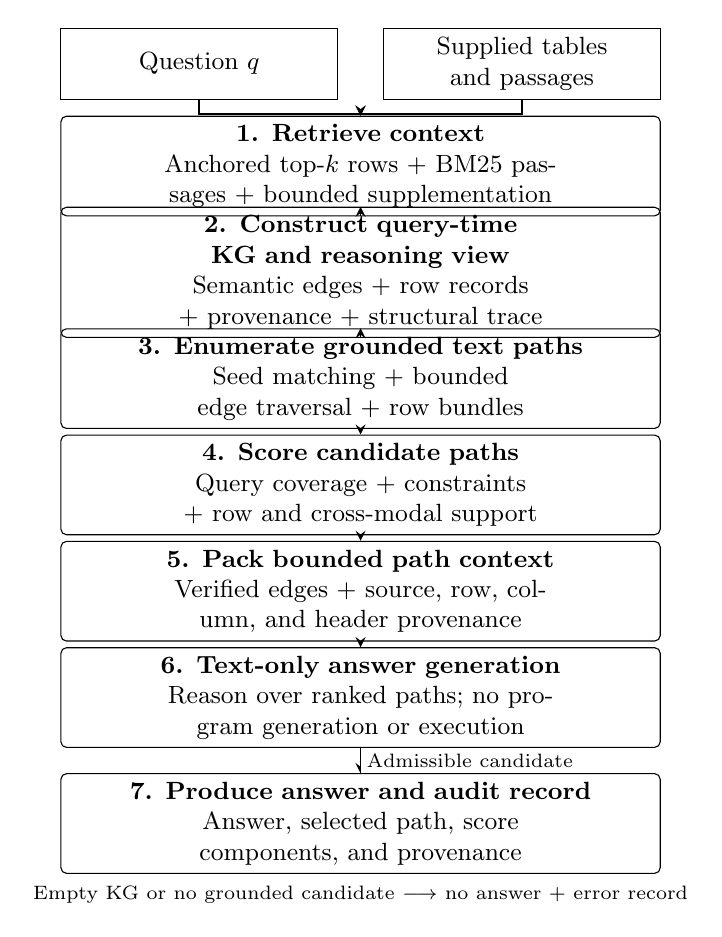
\begin{tikzpicture}[
  >=stealth,
  stage/.style={draw,rounded corners=2pt,align=center,text width=7.4cm,
    minimum height=9mm,inner sep=3pt,font=\small},
  source/.style={draw,align=center,text width=3.3cm,
    minimum height=9mm,inner sep=3pt,font=\small},
  flow/.style={->,line width=0.6pt},
  note/.style={font=\scriptsize,align=center,fill=white,inner sep=2pt}
]
\node[source] (question) at (-2.05,0)
  {Question $q$};
\node[source] (sources) at (2.05,0)
  {Supplied tables and passages};

\node[stage] (retrieve) at (0,-1.3)
  {\textbf{1. Retrieve context}\\
   Anchored top-$k$ rows + BM25 passages + bounded supplementation};
\node[stage] (build) at (0,-2.65)
  {\textbf{2. Construct query-time KG and reasoning view}\\
   Semantic edges + row records + provenance + structural trace};
\node[stage] (plan) at (0,-4)
  {\textbf{3. Enumerate grounded text paths}\\
   Seed matching + bounded edge traversal + row bundles};
\node[stage] (synth) at (0,-5.35)
  {\textbf{4. Score candidate paths}\\
   Query coverage + constraints + row and cross-modal support};
\node[stage] (execute) at (0,-6.7)
  {\textbf{5. Pack bounded path context}\\
   Verified edges + source, row, column, and header provenance};
\node[stage] (select) at (0,-8.05)
  {\textbf{6. Text-only answer generation}\\
   Reason over ranked paths; no program generation or execution};
\node[stage] (answer) at (0,-9.65)
  {\textbf{7. Produce answer and audit record}\\
   Answer, selected path, score components, and provenance};

\draw[flow] (question.south) -- ++(0,-0.18) -| (retrieve.north);
\draw[flow] (sources.south) -- ++(0,-0.18) -| (retrieve.north);
\draw[flow] (retrieve) -- (build);
\draw[flow] (build) -- (plan);
\draw[flow] (plan) -- (synth);
\draw[flow] (synth) -- (execute);
\draw[flow] (execute) -- (select);
\draw[flow] (select) -- node[note,right] {Admissible candidate} (answer);

\node[note] at (0,-10.55)
  {Empty KG or no grounded candidate $\longrightarrow$ no answer + error record};
\end{tikzpicture}
